\section{Exploration and Organization}
\label{sec:exploration}

A rapidly growing number and variety of digital 3D models are becoming available
via large online repositories (e.g. TurboSquid, Trimble 3D Warehouse, etc.).
These repositories can easily archive millions of 3D models covering hundreds of object classes.
%
A key benefit of the accessibility to such model collections is \emph{content reuse} which can greatly simplify the
process of 3D content creation (see Section~\ref{sec:interactive_modeling}). For example, interactively modeling a 3D environment
is made easy by populating the scene with repository models instead of creating everything from scratch.
Another typical scenario is object modeling by retrieving and assembling parts from existing models~\cite{Funkhouser:2004:MBE}.
A common requirement to these tasks is the efficient retrieval of relevant models that may contribute its parts or whole shape
to the modeling. Therefore, a powerful means of exploring the shape variations across the entire collection is indispensable.

Most existing repositories only support text-based model retrieval. However, text-based retrieval often suffers from
the inaccurate and ambiguous semantic tags of the 3D models.
Furthermore, text-based search does not allow exploring the geometric and stylistic variations
in shape collections, since model tag cannot express such information clearly~\cite{Ovsjanikov:2011:ECV,Fisher:2011:CSR}.
For instance, the user may want a chair with short back and long legs.
%
To this end, many works have been devoted to enhancing the retrieval interface to support efficient exploration by learning
the geometric and/or topological variations within the collection, helping the user to better understand and utilize the models therein.
With the learned variations and mutual relations between different shapes,
some works studied the organization of shape collections through grouping and relating the shapes in a systematic way.
Combing with effective visualization, such organization can provide a global view of the entire database~\cite{Huang:2013:QOC}.

\paragraph*{Problem statement and method categorization.}
Data exploration and organization is a classical problem in data analysis and visualization~\cite{Paulovich:2011:PLP}.
Given a data collection, it studies how to \emph{group and relate data points via data comparison}~\cite{Oliveira:2003:VDE},
and (optionally) \emph{organize the data collection into some structured form},
to facilitate retrieval, browsing, summarization, and visualization of the data, based on efficient \emph{interfaces or or metaphor}.
%Most approaches work with feature space and project data
%from the high-dimensional feature space to a low-dimensional visual space for the purpose of visualization and interactive exploration.
The key is the manner to to compare different data points.
This problem has been well studied for image data due to the high demand of
exploring the huge collections of digital images~\cite{Cooper:2005:QOC,Snavely:2006:PT},
aiming to group semantically related images based on some similarity measure~\cite{Nguyen:2008:IAL}.

For 3D models, shape comparison must account for both geometry and topology~\cite{Tangelder:2008:SCB}.
This is especially challenging for complex models, e.g. 3D scenes~\cite{Xu:2014:OHSC},
and heterogeneous model collections encompassing many shape categories~\cite{Huang:2013:QOC}.
%
Generally, any attempt on correlating a set of 3D models via, e.g., finding consistent correspondence across the set,
could be viewed as a kind of organization.
In this section, however, we will only focus on those works targeting at shape variability exploration.
3D shapes should be visually explored within 3D space, which calls for specially designed metaphor.
%
These special requirements of 3D shapes pose several unique problems over the traditional data exploration.
We categorize the existing exploration approaches from four major aspects:
\begin{itemize}
\item \textbf{Shape comparison:} How are the shapes compared (e.g. based on shape similarity or shape correspondence)?
\item \textbf{Variability:} What kind of shape variability can be explored (e.g., geometry, topology, or both)?
\item \textbf{Metaphor:} How are the shape collections explored (e.g. via template or painted ROI)?
\item \textbf{Organization form:} How are the shape collections organized (e.g., into clusters or hierarchies, if available)?
\end{itemize}
Table~\ref{tab:exploration} summarizes several representative works in terms of the above four aspects.
In what follows, we provide detailed review for the recent works, categorized by the first aspect, i.e.,
how the shapes are compared and correlated? Besides traditional shape similarity and shape correspondence,
two unique similarity measures designed for heterogeneous shapes and complex scenes, respectively, are also discussed.

\begin{table}[!t]
\centering
\begin{tabular}{l||c|c|c|c} \hline
                                         & \textbf{Comp.} & \textbf{Var.}  & \textbf{Meta.}  & \textbf{Org.}
 \\ \hline   \cite{Ovsjanikov:2011:ECV}  & simi. & geom. & temp.  & n/a
 \\ \hline   \cite{Kim:2012:FC}          & point & both  & ROI    & n/a
 \\ \hline   \cite{Kim:2013:LPT}         & point & both  & temp.  & cluster
 \\ \hline   \cite{Rustamov:2013:SD}     & point & geom. & ROI    & n/a
 \\ \hline   \cite{Huang:2014:FMN}       & point & both  & ROI    & cluster
 \\ \hline   \cite{Fish:2014:MR}         & part  & geom. & plot    & cluster
 \\ \hline   \cite{Huang:2013:QOC}       & simi. & both  & query  & hierarchy
 \\ \hline   \cite{Xu:2014:OHSC}         & simi. & topo. & ROI    & cluster
 \\ \hline
\end{tabular}
\caption{A summary of several recent works over four aspects.
         Shape \underline{Comp}arison: shape \underline{simi}larity, \underline{part} or \underline{point} correspondence.
         \underline{Var}iability: \underline{geom}etry, \underline{topo}logy or \underline{both}.
         \underline{Meta}phor: \underline{temp}lates, surface painted \underline{ROI}s,
         probability distribution \underline{plot}s, or \underline{query} shapes.
         \underline{Org}anization Form: \underline{cluster} or \underline{hierarchy}.
         For scene exploration, topology refers to structural graphs about scene layout~\cite{Xu:2014:OHSC}.}
\label{tab:exploration}
\end{table}


\paragraph*{Shape descriptor.}
%Sketch-based interface has been adopted for 3D shape retrieval for decades and
%the recent work of Eitz et al.~\shortcite{Eitz:2012:SBS} achieves the state-of-the-art performance.
%Motivated by the ShadowDraw system~\cite{Lee:2011:SD}, which provides data-driven assistance for freehand sketching through exploring
%a database of shadow images with the user's ongoing sketch,
Perhaps the most straightforward approach to shape collection exploration is direct shape retrieval where shapes are
compared based on some kind of shape descriptor~\cite{Tangelder:2008:SCB}.
%
Sketch-based interface has been adopted for 3D shape search for decades and
the recent work of Eitz et al.~\shortcite{Eitz:2012:SBS} achieves the state-of-the-art retrieval performance
based on a novel bag-of-word feature for multi-view line drawings of 3D shapes.
The a sketch-based 3D modeling system of Xie et al.~\shortcite{Xie:2013:S2D} allows the user to create
a 3D model by sketching its parts and exploring a 3D model database to seek for
relevant shape parts for assembly-based modeling.
We are not aware of any work that utilizes sketch-based metaphor to explore shape variability of a model collection.
This is mainly because it is uneasy to modify a 2D sketch dynamically to generate continuously varying queries for exploratory search.

Ovsjanikov et al.~\cite{Ovsjanikov:2011:ECV} construct component-wise bounding box as template and learn the geometric variability of the components
within a set of similar shapes. To avoid relying on correspondence between shapes, they propose a technique that
converts variability in a descriptor space representation of the collection into a deformation model of the template shape,
under the assumption that the set of shapes lies near a low-dimensional manifold in the descriptor space.

\begin{figure}[t]
\centering
    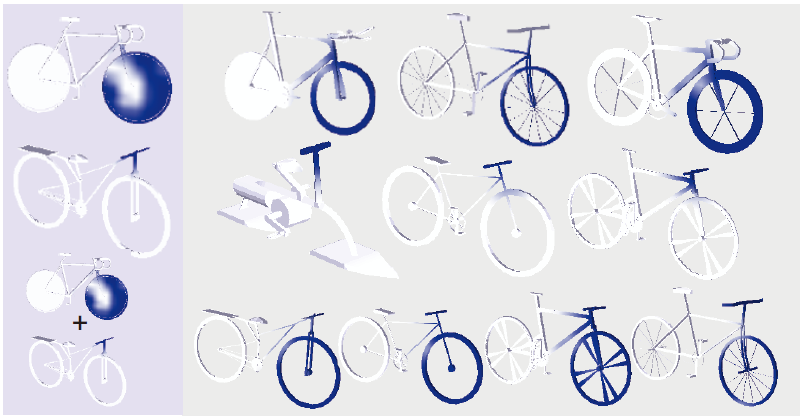
\includegraphics[width=1.0\columnwidth]{fig/img/kim_sig12_fc}
    %\vspace{-0.4cm}
    \caption{Shape exploration based on fuzzy correspondence. The user paints a region of interest (ROI) on a query shape (left column), and the method
    sorts models based on their similarity within the region (right).}
    \label{fig:kim_sig12_fc}
\end{figure}



\paragraph*{Shape correspondence.}
Shape descriptors enable only holistic comparison between shapes or shape parts.
In many cases, the user may prefer to select an arbitrary region on a 3D model and look for more models sharing similar local shape.
Such detailed and flexible query calls for a fine-grained correlation between different shapes, which necessitates correspondences between shapes.
%Some works use a 3D proxy or template to learn the shape variation from 3D models collections
%and allow the user to convey her exploratory intent through interactively deforming the template~\cite{Ovsjanikov:2011:ECV,Kim:2013:LPT}.
%Shape correspondence has been an extensively studied topic in shape analysis~\cite{van-Kaick:2010:SSC}.
%For the task of exploration, however, automatically establishing either part or point correspondences
%across a model collection is difficult and often ambiguous, due to the diverse shape geometry and topology in the collection~\cite{Xu:2010:SCS,Kim:2012:FC}.

Kim et al.~\cite{Kim:2012:FC} propose fuzzy point correspondences to encode the inherent ambiguity
in relating the diverse shapes and estimate the fuzzy correspondences using only a sparse set of pairwise model alignments.
Such dense correspondence supports painting based interface which allows the user
to browse collections based on similarities between shapes in user-specified regions of interest (ROI); see Figure~\ref{fig:kim_sig12_fc}.
%
To learn part-based templates for a large collection of 3D shapes, Kim et al.~\cite{Kim:2013:LPT} propose an algorithm that starts
with an initial template model and then jointly optimizes for part segmentation, point-to-point surface correspondence, and a compact
deformation model to best explain the input collection.
The output is \emph{a set of templates} that groups the input models into clusters capturing their styles and variations.
%
Starting with a map between two shapes, Rustamov et al.~\cite{Rustamov:2013:SD} derive a shape difference operator
revealing detailed information about the location and nature of the differences between the two 3D shapes.
Such detailed comparison can facilitate fine-grained varability exploration of shape collections.
%
Recently, Huang et al.~\cite{Huang:2014:FMN} propose to construct consistent functional maps for shape collections
that exhibit large geometric and topological variability.
The resulting functional maps can be applied to compute shape difference operator~\cite{Rustamov:2013:SD} for
exploring shape collections.

Fish et al.~\cite{Fish:2014:MR} study the configurations of shape parts that are common across a shape family
and express such knowledge with a set of geometric distributions that encode relative arrangements of parts.
To learn the distributions of part arrangement statistically, all shapes in the family are pre-segmented with consistent part correspondence.
The resulting set of probabilistic density functions (PDF) characterize the variability of relations and arrangements
across different parts. A peak in a PDF curve represents a configuration of the related parts
frequently appeared among several shapes in the family.
The multiple PDFs can be used as interfaces to interactively explore the shape family from various views.

\begin{figure}[t]
\centering
    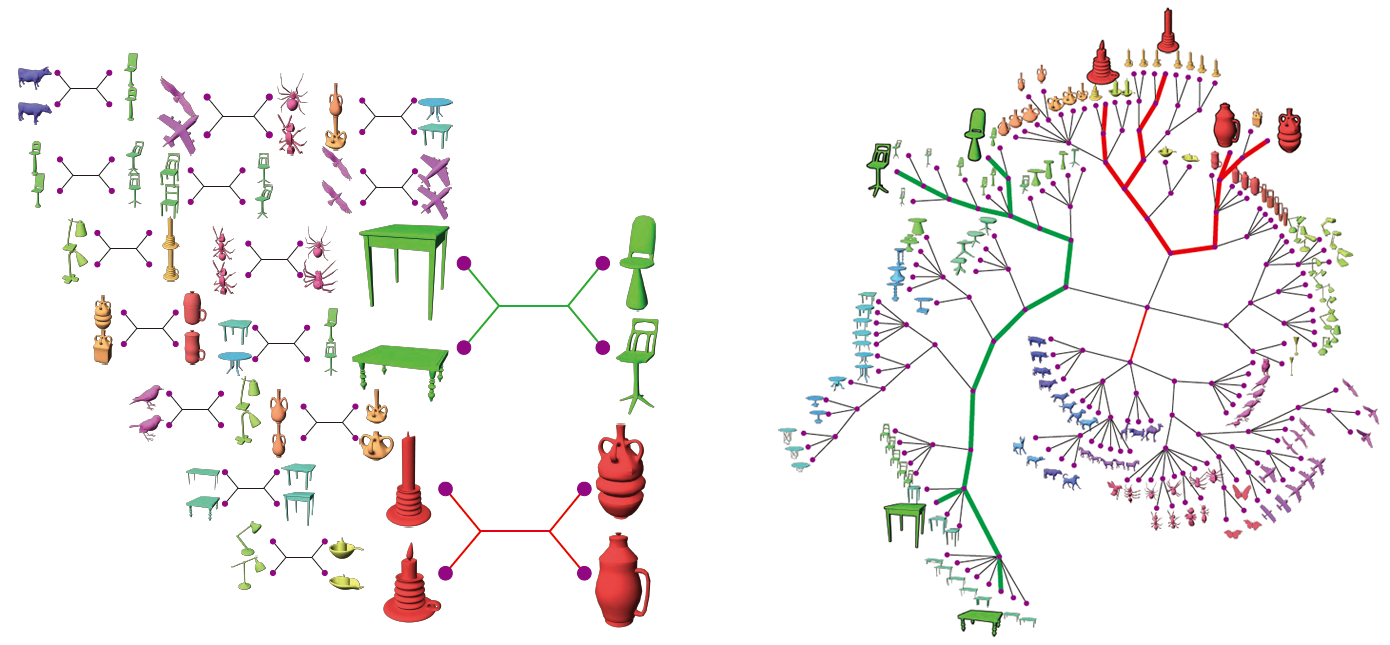
\includegraphics[width=1.0\columnwidth]{fig/img/huang_sig12_quartet}
    %\vspace{-0.4cm}
    \caption{Given a set of heterogeneous shapes, a reliable qualitative similarity is derived from quartets composed of two pairs of objects (left).
    Aggregating such qualitative information from many quartets computed across the whole set leads to a categorization tree as a hierarchical
    organization of the input shape collection (right).}
    \label{fig:huang_sig12_quartet}
\end{figure}



\paragraph*{Qualitative similarity.}
%In general, comparing shapes from different object classes is an ill-posed problem. Therefore,
For a heterogeneous shape collection encompassing diverse object classes, neither shape similarity measuring
nor shape correspondence finding is tractable, making the organization and exploration especially difficult.
To alleviate that, Huang et al.~\cite{Huang:2013:QOC} introduce qualitative analysis from the bioinformatics field.
Rather than relying on quantitative distances, which may be unreliable between dissimilar shapes,
the method considers more reliable \emph{qualitative similarity} derived from \emph{quartets} composed of two pairs of objects.
In each pair, the shapes are close to each other, but far apart from the shapes of the other pair.
%, based on several distance measures.
Aggregating such topological information from many quartets computed across a shape collection, a \emph{categorization tree}
for the collection can be constructed (Figure~\ref{fig:huang_sig12_quartet}).
Analogous to the phylogenetic trees of species, the categorization tree of a shape collection provides an overview of the shapes
about their mutual distance and hierarchical relations.
Based on such organization, they also define the degree of separation chart for every shape in the collection
and apply it for interactive shapes exploration.

\paragraph*{Perspective similarity.}
Recent works on organizing and exploring 3D visual data have been devoted to object collections, with an exception
of the work by Xu et al.~\cite{Xu:2014:OHSC}. The analysis of scenes is known to be more difficult than that of single object.
This is because a scene can easily contain tens to hundreds of objects and scene objects usually suffer from loose
semantic labeling and structural coupling, rendering its structure-aware comparison more challenging.
Fisher et al.~\shortcite{Fisher:2012:CSR} propose a global similarity measure for 3D indoor scenes based on graph kernel,
which can be applied for scene retrieval and context-based object retrieval. For exploration, however, a more fine-grained correlation is demanded.
%
Xu et al.~\cite{Xu:2014:OHSC} advocate that 3D scenes should be compared from the \emph{perspective} of a particular
focal point which is a representative substructure of a specific scene category.
Focal points are detected through contextual analysis of a collection of scenes, resulting in a clustering
of the scene collection where each cluster is characterized by its representative focal points (see Section~\ref{sec:scene}).
%
Consequently, the focal points extracted from a scene collection can be used to organize collection into an interlinked and well-connected cluster
formation, which facilitates scene exploration. Figure~\ref{fig:xu_sig14_expl} shows an illustration of such cluster-based organization
and an exploratory path transiting between two scene clusters/categories.


%\teaser{
\begin{figure}[t]
\centering
    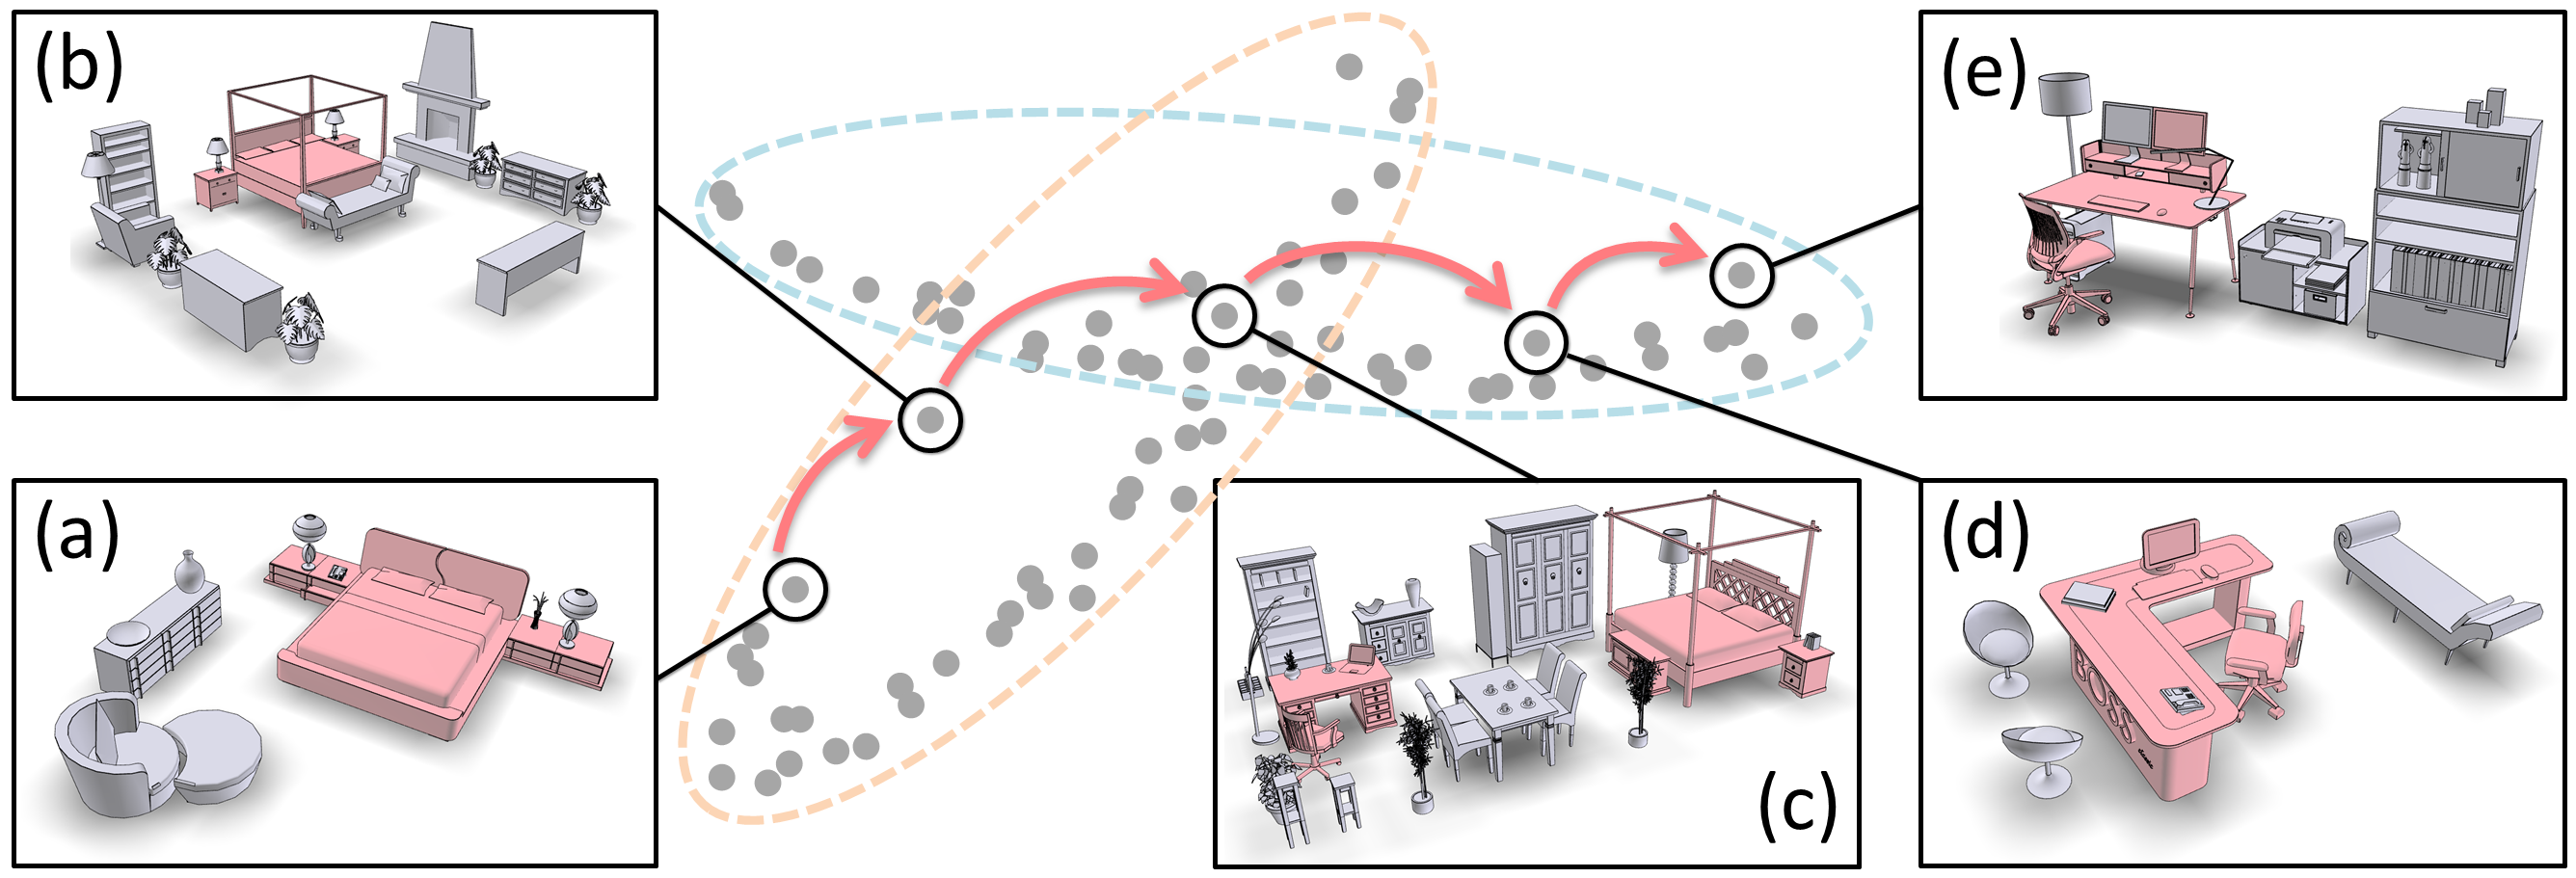
\includegraphics[width=0.99\linewidth]{fig/img/xu_sig14_expl}
%    \vspace{-0.4cm}
    \caption{
    Focal-based scene clustering produces overlapping clusters, which is due to hybrid scenes possessing multiple focal points.
    An exploratory path, from (a) to (e), through the overlap, smoothly transit between the two scene clusters,
    representing bedroom and offices, respectively.}
    \label{fig:xu_sig14_expl}
\end{figure}
%}

